\documentclass[10pt]{beamer}

\usetheme{metropolis}
\usepackage{appendixnumberbeamer}

\usepackage{booktabs}
\usepackage[scale=2]{ccicons}

\usepackage{pgfplots}
\usepgfplotslibrary{dateplot}

\usepackage{xspace}
\usepackage{bm}
\newcommand{\themename}{\textbf{\textsc{metropolis}}\xspace}

\usepackage{amsmath}
\DeclareMathOperator*{\argmin}{arg\,min}

\title{Mid-term Project}
\subtitle{Chan and Ho: A Simple and Efficient Estimator for Hyperbolic Location System}
\date{\today}
\author{Zhang Niansong\quad(16308149) \\ Yang Songyi\quad(16308131)}
\titlegraphic{\hfill
\includegraphics[height=1.5cm]{logo.pdf}}

\begin{document}

\maketitle

\begin{frame}{Table of contents}
  \setbeamertemplate{section in toc}[sections numbered]
  \tableofcontents[hideallsubsections]
\end{frame}


\section{Introduction}

\begin{frame}{Position Fix by TDOA}
  \begin{columns}[T,onlytextwidth]
    \column{0.6\textwidth}
      \begin{itemize}
        \item Assuming a source is emitting signal in all directions
              and an array of sensors are picking up the signal,
              it will arrive at different sensors at different time.
        \item \textbf{TDOA :} \textit{Time Difference Of Arrival}
        \item Then the location of the source can be estimated
              by measuring the delay of signal arriving at different sensor.
      \end{itemize}
    \column{0.3\textwidth}
      \begin{figure}[t]
        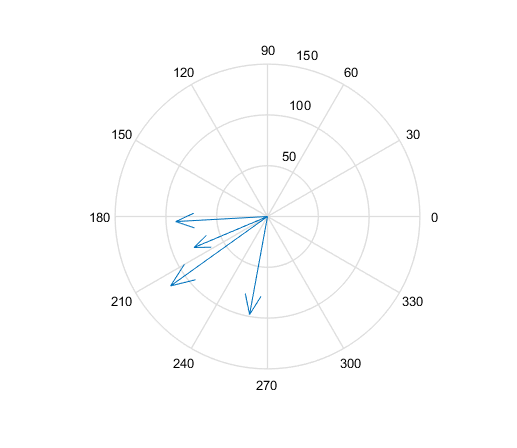
\includegraphics[width=1\textwidth]{intro.png}
        \caption{Sensors and source.}
      \end{figure}
  \end{columns}
\end{frame}

\begin{frame}{Position Fix by TDOA: Noise}
  Vector of \textbf{TDOA}:
    $$\bf{d} = \begin{bmatrix} d_2-d_1 & d_3-d_1 & \cdots \end{bmatrix}^\it{T}$$
  However, 100\% precise measurement of \textbf{TDOA} is not possible.
  Noise is always present.

  Naturally, the noise in \textbf{TDOA} is a \textit{multivariate Gaussian distribution}
  centered at true value, with covariance given by matrix:
    $$ \mathbf{Q} = \sigma^2
      \begin{bmatrix}
        1 & 0.5 & \cdots & 0.5 \\
        0.5 & 1 & \cdots & 0.5 \\
        \vdots & \vdots & \ddots & \vdots \\
        0.5 & 0.5 & \cdots & 1 \end{bmatrix}
    $$
    where $\sigma^2$ is the noise power.
\end{frame}

\section{Propsed Method}

\begin{frame}{Proposed Method}
  \begin{itemize}[<+- | alert@+>]
    \item By assuming $x, y$ and $r_1$ are independent, the non-linear
          equations can be reduced into linear ones.

    \item Given different situations, use \emph{Maximum Likelihood} (ML)
          estimator to solve the linear equations.

    \item Incorporate the dependent relationship back into the solution (if necessary)
          to get more accurate solution.

  \end{itemize}
\end{frame}

\begin{frame}{Proposed Method: Workflow}

  \begin{figure}
    \centering
    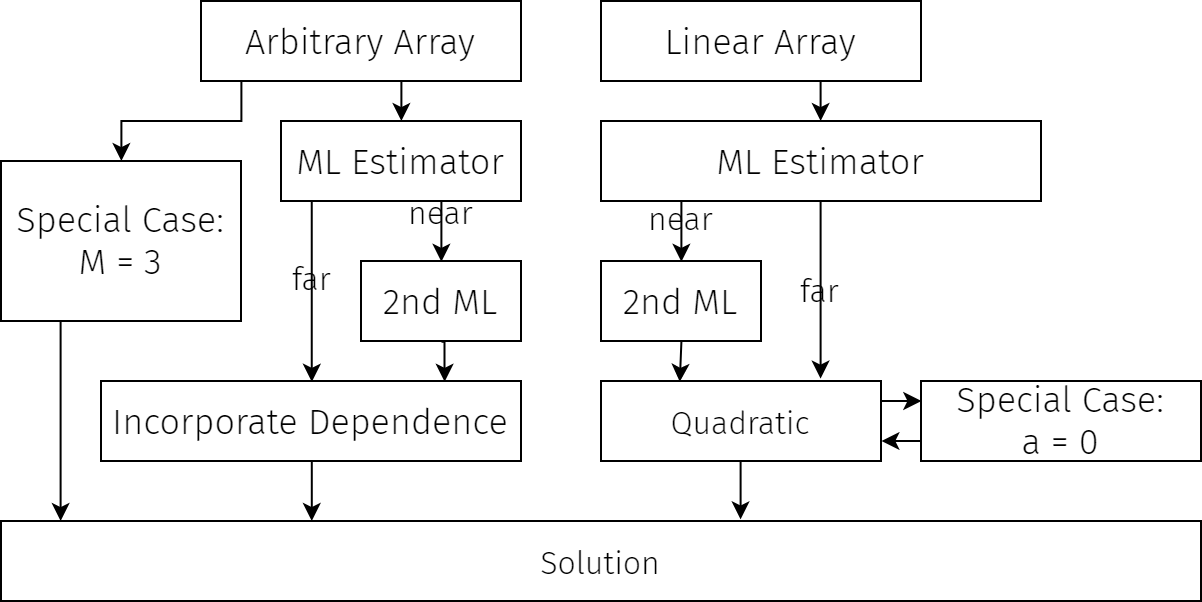
\includegraphics[width=0.9\textwidth]{proposed-workflow.png}
    \caption{Flowchart of the proposed method.}
  \end{figure}
\end{frame}

\begin{frame}{Proposed Method: Arbitrary Array}
  "Arbitrary" refers to that sensors are arranged in a non-linear manner,
  thus avoiding singularity during computation.
  \begin{itemize}
    \item With \alert{3} sensors ($M = 3$), system is not overdetermined.
            $$\mathbf{z}_p = - \begin{bmatrix}x_{2,1}&y_{2,1} \\ x_{3,1}&y_{3,1}\end{bmatrix}^{-1} \times
              \begin{Bmatrix} \begin{bmatrix}r_{2,1}\\r_{3,1}\end{bmatrix}r_1 + \frac{1}{2}
                              \begin{bmatrix}r_{2,1}^2-K_2+K_1 \\ r_{3,1}^2-K_3+K_1 \end{bmatrix}\end{Bmatrix}$$
            $$r_1^2 = K_1-
              2\begin{bmatrix}x_1&y_1\end{bmatrix} \mathbf{z}_p+
              \mathbf{z}_p^T \mathbf{z}_p$$
          where $K_i = x_i^2 + y_i^2, \mathbf{z}_p = \begin{bmatrix}x&y\end{bmatrix}^T$.
    \item Therefore, the solution can be found simply by
    \begin{enumerate}
      \item solving a quadratic equation of $r_1$;
      \item insert $r_1$ back and solve the linear equation groups of $x$ and $y$.
    \end{enumerate}
  \end{itemize}
\end{frame}

\begin{frame}{Proposed Method: Arbitrary Array (cont'd)}
  \begin{itemize}
    \item With more than 3 sensors, the system is overdetermined.
    \item Here we denote:
            $$\mathbf{h}= \frac{1}{2}
              \begin{bmatrix}r_{2,1}^2-K_2+K_1 \\
                             r_{3,1}^2-K_3+K_1 \\
                             \vdots \\
                             r_{M,1}^2-K_M+K_1\end{bmatrix}$$
            $$\mathbf{G}_a=-
              \begin{bmatrix} x_{2,1} & y_{2,1} & r_{2,1} \\
                              x_{3,1} & y_{3,1} & r_{3,1} \\
                              \vdots  & \vdots  & \vdots  \\
                              x_{M,1} & y_{M,1} & r_{M,1} \end{bmatrix}$$
            $$\mathbf{B}= \textbf{diag} \{r_2^0,r_3^0,\cdots,r_M^0\}$$
    \item
  \end{itemize}
\end{frame}

\begin{frame}{Proposed Method: Arbitrary Array (cont'd)}
  \begin{itemize}
    \item Using ML estimator, $\mathbf{z}_a=\begin{bmatrix}x\\y\\r_1\end{bmatrix}$ can be obtained as
          $$\begin{align}
            \mathbf{z}_a&=\argmin\{(\mathbf{h}-\mathbf{G}_a\mathbf{z}_a)^T
                                    \Psi^{-1}(\mathbf{h}-\mathbf{G}_a\mathbf{z}_a)\}\\
                        &=(\mathbf{G}_a^T\Psi^{-1}\mathbf{G}_a)^{-1}\mathbf{G}_a^T\Psi^{-1}\mathbf{h}
            \end{align}$$
    \item When the emitter is far away from the sensors,
          and since scaling of $\Psi$ do not effect the solution
          $\mathbf{z}_a$can be approximated as
          $$\mathbf{z}_a\approx(\mathbf{G}_a^T\mathbf{Q}^{-1}
            \mathbf{G}_a)^{-1}\mathbf{G}_a^T\mathbf{Q}^{-1}\mathbf{h}$$
    \item When the source is nearby, its location can still be approximated
          using $\mathbf{Q}$, and using one iteration to improve accuracy.
  \end{itemize}
\end{frame}

\begin{frame}{Proposed Method: Dependency of Arbitrary Array}
  \begin{itemize}
    \item The next step is to consider the dependency between $x$, $y$ and $r_1$.
    \item Again using ML, we have
          $$\mathbf{z}_a^{'}=(\mathbf{G}_a^{'T}\Psi^{'-1}\mathbf{G}_a^{'})^{-1}
                              \mathbf{G}_a^{'T}\Psi^{'-1}\mathbf{h}^{'}$$
          where
          $$\mathbf{h}^{'}=\begin{bmatrix}(x-x_1)^2\\(y-y_1)^2\\r_1^2\end{bmatrix},\quad
            \mathbf{G}_a^{'}=\begin{bmatrix}1&0\\0&1\\1&1\end{bmatrix}$$
          and
          $$\Psi^{'}=4\mathbf{B}^{'}(\mathbf{G}_a^{0T}\Psi^{-1}\mathbf{G}_a^0)^{-1}\mathbf{B}^{'},\quad
            \mathbf{B}^{'} = \textbf{diag} \{x-x_1,y-y_1,r_1^0\}$$
  \end{itemize}
\end{frame}

\begin{frame}{Proposed Method: Solution of Arbitrary Array}
  \begin{itemize}
    \item Similar simplification can be made when the source is far away,
          by subsitituding $\Psi$ with $\mathbf{Q}$.
    \item After acquiring $\mathbf{z}_a^{'}$, we have
          $$\mathbf{z}_a^{'}=
            \begin{bmatrix}(x^0-x_1)^2\\(y^0-y_1)^2\end{bmatrix}$$
    \item Then $x^0$ and $y^0$ can be canculated by taking square roots of the positive values.
  \end{itemize}
\end{frame}

\begin{frame}{Proposed Method: Linear Array}
  If the sensors are arranged linearly, i.e. on a line, then the positions
  can be described by $$y=ax+b$$

  Here the procedure used for \emph{Arbitrary Array} would fail due to matrix singularity.

  However, a similar solution can be developed with slight modifications.
\end{frame}

\begin{frame}{Proposed Method: Linear Array (cont'd)}
  \begin{itemize}
    \item Taking the relationship $y=ax+b$, rewrite $\mathbf{z}_a$ and $\mathbf{G}_a$
          as
          $$\mathbf{z}_l=\begin{bmatrix}x+ay\\r_1\end{bmatrix},\quad
            \mathbf{G}_l=-\begin{bmatrix}
                          x_{2,1} & r_{2,1}\\
                          x_{3,1} & r_{3,1}\\
                          \vdots  & \vdots \\
                          x_{M,1} & r_{M,1}\end{bmatrix}$$
    \item We can have something very similar to that in arbitrary array
          $$\mathbf{z}_l=(\mathbf{G}_l^T\Psi^{-1}\mathbf{G}_l)^{-1}\mathbf{G}_l^T\Psi^{-1}\mathbf{h}$$
          where $\Psi$ and $\mathbf{h}$ are the same as in arbitrary Array.
    \item Similar approach of taking $\mathbf{Q}$ for $\Psi$ and use of iteration can be applied here.
  \end{itemize}
\end{frame}

\begin{frame}{Proposed Method: Solution of Linear Array}
  We now have $\mathbf{z}_l=\begin{bmatrix}x+ay\\r_1\end{bmatrix}$,
  denoted as $\mathbf{z}_l=\begin{bmatrix}w\\r_1\end{bmatrix}$.
  \begin{itemize}
    \item $y$ and $x$ can be solved through quadratic equation
          $$y=\frac{-E\pm\sqrt{E^2-4AC}}{2A},\quad x=w-ay$$
          where$$A=1+a^2,E=-2(aw+b),C=K_1-2x_1w+w^2-r_1^2$$
    \item When $a=0$, the solution becomes
          $$y=\pm\sqrt{r_1^2-(w-x_1)^2}+y_1,\quad x=w$$
  \end{itemize}
\end{frame}

%-----------------------Taylor-series Method--------------------------------------
\section{Taylor-series Method}

\begin{frame}{Taylor-Series Method}
	We are given:
  $$ r_{i,1}=cd_{i,1}=r_{i}-r_{1} $$
  Linearize above equation by Taylor-series expansion and then solve iteratively:
	\begin{itemize}
    \item Compute position deviation
    \item Add position deviation to initial guess
    \item Solve again until deviation is considerably small
  \end{itemize}
  \alert{Convergence is not guaranteed}
\end{frame}


\begin{frame}{Taylor-series Method}
	The position deviation is computed by:
   $$\begin{bmatrix} \Delta x \\ \Delta y \end{bmatrix} = (\mathbf{G_{t}^T Q^{-1} G_{t})^{-1} G_{t}^T Q^{-1} h_{t}}$$
  where $h_{t}$ and $G_{t}$ are given as follows
 \begin{align}
    \mathbf{h_{t}} &= \begin{bmatrix} r_{2,1} - (r_{2}-r_{1}) \\  r_{3,1} - (r_{3}-r_{1})\\  \quad\\  r_{M,1} - (r_{M}-r_{1}) \end{bmatrix}  \\
    \mathbf{G_{t}} &= \begin{bmatrix} (x_{1}-x)/r_{1} - (x_{2}-x)/r_{2} & (y_{1}-y)/r_{1} - (y_{2}-y)/r_{2} \\ (x_{1}-x)/r_{1} - (x_{2}-x)/r_{3} & (y_{1}-y)/r_{1} - (y_{3}-y)/r_{3}\\  \quad\\ (x_{1}-x)/r_{1} - (x_{M}-x)/r_{M} & (y_{1}-y)/r_{1} - (y_{M}-y)/r_{M} \end{bmatrix}
  \end{align}

\end{frame}

%------------------------Spherical Interpolation Method-------------------------------
\section{Spherical-Interpolation Method}

% page 1
\begin{frame}{The Equation-Error Formulation}
  We first map the spatial origin to an arbitrary sensor j, this gives:
  $$ \mathbf{\underline{x}_{j}}\triangleq \underline{0}\Longrightarrow \begin{cases} R_{j} &= \ 0 \\ D_{j} &= \ R_{s} \end{cases}$$
  From the Pythagorean theorem, we have:
  $$(R_{s}+d_{ij})^2 = R_{i}^2 - 2\mathbf{\underline{x}_{i}^T \underline{x}_{s}} + R_{s}^2 $$
  which is also:
  $$ 0 = R_{i}^2 - d_{ij}^2 -2R_{s}d_{ij} - 2\mathbf{\underline{x}_{i}^T \underline{x}_{s}} $$
  \begin{center}
  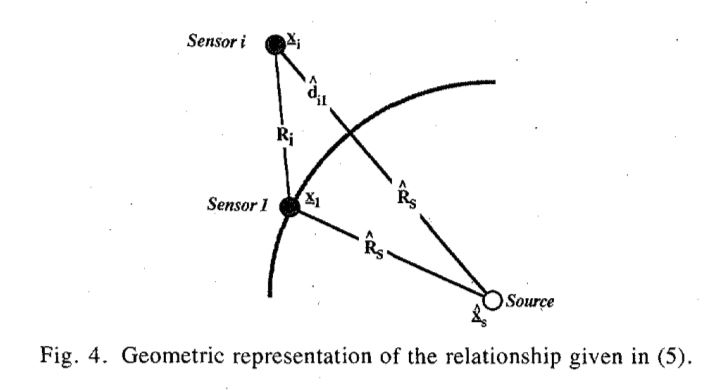
\includegraphics[scale=0.7]{Pythagorean.JPG}
  \end{center}
\end{frame}
% page 2
\begin{frame}{The Equation-Error Fomulation}
  If we take the first sensor as origin, i.e. $j=1$ \\
  As the delays are typically not measured precisely, we introduce "equation error"
  $$ \epsilon_{i} = R_{i}^2 - d_{ij}^2 -2R_{s}d_{ij} - 2\mathbf{\underline{x}_{i}^T \underline{x}_{s}} \quad (i=2,3,\ldots,N) $$
  where $\epsilon_{i}$ is to be minimized.
  With N-1 measurements, this equation can be written in matrix notaion:
  $$ \boldsymbol{\underline{\epsilon}} = \boldsymbol{\underline{\sigma}} - 2R_{s}\mathbf{\underline{d}} - 2 \mathbf{ S \cdot \underline{x}_{s}} $$
  where
  \begin{align*}
    \boldsymbol{\underline{\sigma}} \triangleq \begin{bmatrix} R_{2}^2 - d_{21}^2 \\ R_{3}^2 - d_{31}^2 \\ \vdots \\ R_{N}^2 - d_{N1}^2 \end{bmatrix} \qquad
    \mathbf{\underline{d}}      \triangleq \begin{bmatrix} d_{21}\\ d_{31} \\ \vdots \\ d_{N1} \end{bmatrix} \qquad
    \mathbf{S} \triangleq \begin{bmatrix} x_2 & y_2 \\x_3 & y_3\\ \vdots & \vdots \\ x_N & y_N \end{bmatrix}
  \end{align*}
\end{frame}
% page 3
\begin{frame}{The Spherical-Interpolation Method}
  The formal least-squares solution for $\mathbf{\underline{x}_s}$ \alert{given} $R_s$ is
  $$ \mathbf{\underline{x}_s }= \frac{1}{2} \mathbf{S_W^*} (\boldsymbol{\underline{\sigma}} - 2R_s\mathbf{\underline{d}})$$
  where
  $$  \mathbf{S_W^* \triangleq (S^T S)^{-1}S^T} $$
  The \alert{SI} method is to minimize the equation error agian with respect to $R_s$.
  i.e. rewriting the equation error to eliminate $\underline{x}_s$ by substituting it with $R_s$, yielding a new equation error $\underline{\epsilon}^{'}$ which is linear in $R_s$:
  \begin{align*}
   \boldsymbol{\underline{\epsilon}^{'}} &= \boldsymbol{\underline{\sigma}} - 2R_s\mathbf{\underline{d} - S S^*_W (\boldsymbol{\underline{\epsilon}}} - 2R_s\mathbf{\underline{d}})\\
                            &= \mathbf{(I - S S_W^*)}(\boldsymbol{\underline{\epsilon}} - 2R_s\mathbf{\underline{d}})
  \end{align*}
  We notice that the formal least-squares estimate of  $\mathbf{\underline{x}_s}$ \alert{given} $R_s$ is itself \textsc{linear} in $R_s$. When the minimizing $R_s$ value is found
  in this new equation, the corresponding value of $\mathbf{\underline{x}_s}$ is automatically a minimizer of the squared equation-error norm.
\end{frame}
% page 4
\begin{frame}{The Spherical-Interpolation Method}
  The solution is given by
  $$ \mathbf{\tilde{R}_s = \frac{\underline{d}^T P_s^{\bot}V P_s^{\bot}\boldsymbol{\underline{\sigma}}}{2\underline{d}^T P_s^{\bot} V P_s^{\bot}\underline{d}}}$$
  where $\mathbf{P_s^{\bot}}$ is defined as
  $$\mathbf{P_s^{\bot} \triangleq I - SS_W^*}$$
  Substituting this solution into
  $$  \mathbf{\underline{x}_s }= \frac{1}{2} \mathbf{S_W^*} (\boldsymbol{\underline{\sigma}} - 2R_s\mathbf{\underline{d}}) $$
  yields the source location estimate
  $$ \mathbf{\hat{\underline{x}}_s} = \frac{1}{2} \mathbf{(S^T W S)^{-1} S^T W (I - \frac{\underline{d}\ \underline{d}^T P_s^{\bot} V P_s^{\bot}} {\underline{d}^T P_s^{\bot} V P_s^{\bot} \underline{d}})} \boldsymbol{\underline{\sigma}} $$
\end{frame}
% page 5
\begin{frame}{The Spherical-Interpolation Method}
  When $\mathbf{W = V}$ , this estimator is the minimizer of the weighted norm of the \alert{projected} equation error
  $$ \mathbf{Z_{\underline{x}_s} = \boldsymbol{\underline{\epsilon}}^T P_{\underline{d}}^{\bot} W P_{\underline{d}}^{\bot} \boldsymbol{\underline{\epsilon}} }$$
  Minimizing $Z_{\underline{x}_s}$, one gets a simplified expression of the estimator
  $$ \mathbf{\hat{\underline{x}}_s} = \frac{1}{2} \mathbf{(S^T  P_{\underline{d}}^{\bot} W P_{\underline{d}}^{\bot} S)^{-1} S^T P_{\underline{d}}^{\bot}} \boldsymbol{\underline{\sigma}} $$
  By now, the \alert{Maximum Likelihood Estimation} of the $\mathbf{\underline{x}_s}$ is obtained.
  \vfill
  \textsc{in simulation:\\}
  The weighting matrices $\textbf{W}$ and $\textbf{V}$ are both set to $\textbf{Q}^{-1}$
\end{frame}

%----------------------------------------CRLB-----------------------------------------
\section{Cram\'{e}r-Rao Lower Bound}

% page 1
\begin{frame}{Cram\'{e}r-Rao Lower Bound}
  In the simplest form, the CRLB states that the variance of any unbiased estimator
  is no smaller than the inverse of the Fisher information matrix.
   $$\textbf{var}(\hat{\theta}) \geqslant \textbf{J}(\theta)^{-1} $$
  It is derived from the \textsc{appendix} that the CRLB of the localization problem
  is given by
   $$ \bm{\Phi^0} = c^2 (\textbf{G}_t^{0T} \textbf{Q}^{-1} \textbf{G}_l^0)^{-1} $$
  Also, it is proved that the proposed method with arbitrary sensor array can achieve CRLB,
  therefore, one can use the following method to compute the lower bound of covariance matrix
  \begin{align*}
    \boldsymbol{\Phi^0} &= \text{cov}(\textbf{z}_p) = \frac{1}{4} \textbf{B}^{''-1} \text{cov} (\textbf{z}_a^{'}) \textbf{B}^{''-1} \\
           &= c^2 ( \textbf{B}^{''} \textbf{G}_a^{'T} \textbf{B}^{'-1} \textbf{G}_a^{0T} \textbf{B}^{-1} \textbf{Q}^{-1} \textbf{B}^{-1} \textbf{G}_a^{0}  \textbf{B}^{'-1} \textbf{G}_a^{'} \textbf{B}^{''} )^{-1}
  \end{align*}
  which is the covariance matrix of $\textbf{z}_p$ when errors are ignored.
  \begin{center}
    \textsc{Predefined matrices are given in the next slide}
  \end{center}
\end{frame}
% page 2
\begin{frame}{Cram\'{e}r-Rao Lower Bound}
  \begin{equation*}
    \boldsymbol{\Phi^0} = c^2 ( \textbf{B}^{''} \textbf{G}_a^{'T} \textbf{B}^{'-1} \textbf{G}_a^{0T} \textbf{B}^{-1} \textbf{Q}^{-1} \textbf{B}^{-1} \textbf{G}_a^{0}  \textbf{B}^{'-1} \textbf{G}_a^{'} \textbf{B}^{''} )^{-1}
  \end{equation*}
  where
  \begin{align*}
     \textbf{G}_a^0   &= - \begin{bmatrix} x_2  & y_2 & r_2-r_1 \\   x_3  & y_3 & r_3-r_1 \\ \vdots & \vdots & \vdots \\  x_M  & y_M & r_M-r_1 \end{bmatrix} \qquad \qquad
     \textbf{B}^{''}  = \begin{bmatrix} (x^0 - x_1) & 0 \\  0 & (y^0 - y_1)\end{bmatrix}\\
     \textbf{B}^{'}\  &= \text{diag}\{(x^0 - x_1),(y^0 - y_1),r_1^0\}\qquad
     \textbf{G}_a^{'} = \begin{bmatrix} 1 & 0 & 1 \\  0 & 1 & 1\end{bmatrix}^{'} \\
     \textbf{B}  \ \  &= \text{diag}\{r_2^0, r_3^0, \cdots r_M^0\}
   \end{align*}
   The covariance matrix of position estimate contains the uncertainty information in localization.
   In particular, the position mean-square error (\textsc{MSE}) is equal to the \alert{trace} of $\boldsymbol{\Phi}$.
\end{frame}

%-------------------------------Simulation Results------------------------------------
\section{Simulation Results}

%page 1
\begin{frame}{Simulation Results}
  \begin{center}
  \begin{tabular}{l c c c c c c c c}\\
  \multicolumn{9}{c}{TABLE \uppercase\expandafter{\romannumeral1}}\\
  \multicolumn{9}{c}{\textsc{\tiny Comparison of MSE for the SI, Taylor-Series and Proposed Methods; Arbitrary Array and Near Source}}\\\hline
  \scriptsize MSE  &  \scriptsize  M=3     &  \scriptsize  M=4    &  \scriptsize M=5    &  \scriptsize  M=6    &  \scriptsize  M=7    &  \scriptsize M=8    &  \scriptsize M=9     &  \scriptsize M=10     \\\hline
  \scriptsize A    &  \scriptsize no.sol.  &  \scriptsize  1.5741 &  \scriptsize 0.1585 &  \scriptsize  0.1487 &  \scriptsize  0.1241 &  \scriptsize 0.1165 &  \scriptsize 0.1138  &  \scriptsize 0.1106   \\
  \scriptsize B    &  \scriptsize 2.1646   &  \scriptsize  0.7095 &  \scriptsize 0.1463 &  \scriptsize  0.1338 &  \scriptsize  0.1153 &  \scriptsize 0.1059 &  \scriptsize 0.1031  &  \scriptsize 0.0947   \\
  \scriptsize C    &  \scriptsize 2.1701   &  \scriptsize  0.7003 &  \scriptsize 0.1451 &  \scriptsize  0.1411 &  \scriptsize  0.1155 &  \scriptsize 0.1105 &  \scriptsize 0.1050  &  \scriptsize 0.0981   \\
  \scriptsize D    &  \scriptsize 2.1546   &  \scriptsize  0.6854 &  \scriptsize 0.1492 &  \scriptsize  0.1361 &  \scriptsize  0.1150 &  \scriptsize 0.1077 &  \scriptsize 0.1037  &  \scriptsize 0.0961   \\
  \scriptsize E    &  \scriptsize 1.9766   &  \scriptsize  0.6873 &  \scriptsize 0.1448 &  \scriptsize  0.1332 &  \scriptsize  0.1141 &  \scriptsize 0.1052 &  \scriptsize 0.1030  &  \scriptsize 0.0941   \\\hline
  \multicolumn{9}{l}{\tiny A: SI method. B: Taylor series method. C: proposed method, \{ (14b), (22b), (24)\}. D: proposed method, \{(14b),(14a), (22a), (24)\}. }\\
  \multicolumn{9}{l}{\tiny E: theoretical MSE of the new method = CRLB.}
  \end{tabular}
  \end{center}
  %\begin{center} \textsc{Conclusions} \end{center}  % -- deleted because the page is over-crowded
  \begin{itemize}
		\item \small SI performs worst and our solution method gives a slightly smaller MSE than the Taylor-series method.
		%\item \small The differences between the two proposed methods is small.
		\item \small The proposed method with the simplified formulae still performs better than the SI method.
	\end{itemize}
\end{frame}

%page 2
\begin{frame}{Simulation Results}
  \begin{center}
  \begin{tabular}{l c c c c c c c c}\\
  \multicolumn{9}{c}{TABLE \uppercase\expandafter{\romannumeral2}}\\
  \multicolumn{9}{c}{\textsc{\tiny Comparison of MSE for the Proposed and Taylor-Series Methods; Linear Array and Near Source}}\\\hline
  \scriptsize MSE  &   \scriptsize  M=3   &  \scriptsize  M=4    &  \scriptsize M=5    &  \scriptsize  M=6    &  \scriptsize  M=7    &  \scriptsize M=8    &  \scriptsize  M=9     &  \scriptsize  M=10   \\\hline
  \scriptsize B    &   \scriptsize no.sol.&  \scriptsize  1.3342 &  \scriptsize 0.3794 &  \scriptsize  0.1247 &  \scriptsize  0.0618 &  \scriptsize 0.0283 &  \scriptsize  0.0175  &  \scriptsize  0.0096 \\
  \scriptsize C    &   \scriptsize 8.2421 &  \scriptsize  1.1107 &  \scriptsize 0.3563 &  \scriptsize  0.1222 &  \scriptsize  0.0619 &  \scriptsize 0.0286 &  \scriptsize  0.0178  &  \scriptsize  0.0098 \\
  \scriptsize D    &   \scriptsize 8.2289 &  \scriptsize  1.1020 &  \scriptsize 0.3566 &  \scriptsize  0.1219 &  \scriptsize  0.0613 &  \scriptsize 0.0286 &  \scriptsize  0.0174  &  \scriptsize  0.0096 \\
  \scriptsize E    &   \scriptsize 7.2718 &  \scriptsize  1.0984 &  \scriptsize 0.3543 &  \scriptsize  0.1217 &  \scriptsize  0.0611 &  \scriptsize 0.0283 &  \scriptsize  0.0174  &  \scriptsize  0.0095 \\\hline
  \multicolumn{9}{l}{\tiny B: Taylor series method. C: proposed method, \{ (28) with $\Psi = Q$, (29)\}. D: proposed method, \{(28) with $\Psi = Q$, (28),(29)\}. }\\
  \multicolumn{9}{l}{\tiny E: theoretical MSE of the new method = CRLB.}
  \end{tabular}
  \end{center}
  \begin{center} \textsc{Conclusions} \end{center}
  \begin{itemize}
		\item \small The localization MSE decreases as the number of sensor increases.
		\item \small The Taylor-series method gives almost identical results as the new method.
	\end{itemize}
\end{frame}

%page 3
\begin{frame}{Simulation Results}
  \begin{center}
  \begin{tabular}{l c c c c c c c}\\
  \multicolumn{8}{c}{TABLE \uppercase\expandafter{\romannumeral3}}\\
  \multicolumn{8}{c}{\textsc{\tiny Comparison of MSE for the SI, Taylor-Series and Proposed Methods;}}\\
  \multicolumn{8}{c}{\textsc{\tiny Arbitrary Array and Distant Source}}\\\hline
  \scriptsize MSE & \scriptsize  M=4   &  \scriptsize M=5    & \scriptsize  M=6   & \scriptsize  M=7   &  \scriptsize M=8   &  \scriptsize M=9   &  \scriptsize M=10   \\\hline
  \scriptsize A   & \scriptsize  14796 &  \scriptsize 212.10 & \scriptsize  48.16 & \scriptsize  40.70 & \scriptsize  42.02 &  \scriptsize 39.99 &  \scriptsize 37.57  \\
  \scriptsize B   &  \scriptsize 346.52&  \scriptsize 147.50 &  \scriptsize 44.98 &  \scriptsize 38.77 &  \scriptsize 39.40 &  \scriptsize 37.56 &  \scriptsize 33.39  \\
  \scriptsize C   &  \scriptsize 450.65&  \scriptsize 143.92 &  \scriptsize 44.74 &  \scriptsize 38.69 &  \scriptsize 38.53 &  \scriptsize 36.85 &  \scriptsize 34.14   \\
  \scriptsize E   &  \scriptsize 328.36&   \scriptsize 143.73&  \scriptsize 44.00 &  \scriptsize 38.48 &  \scriptsize 38.47 &  \scriptsize 36.41 &  \scriptsize 33.68  \\\hline
  \multicolumn{8}{l}{\tiny A: SI method. B: Taylor series method. C: proposed method, \{ (14b), (22b), (24)\}}\\
  \multicolumn{8}{l}{\tiny E: theoretical MSE of the new method = CRLB.}
  \end{tabular}
  \end{center}
  \begin{center} \textsc{Conclusions} \end{center}
  \begin{itemize}
		\item \small The proposed method performs much better than SI and slightly better than Taylor-series method.
		\item \small The proposed method performs significantly better when M is small.
	\end{itemize}

\end{frame}

% page 4
\begin{frame}{Simulation Results}
  \begin{center}
  \begin{tabular}{l c c c c c c c}\\
  \multicolumn{8}{c}{TABLE \uppercase\expandafter{\romannumeral4}}\\
  \multicolumn{8}{c}{\textsc{\tiny Comparison of MSE for the Proposed and Taylor-Series Methods;}}\\
  \multicolumn{8}{c}{\textsc{\tiny Linear Array and Distant Source}}\\\hline
  \scriptsize MSE & \scriptsize  M=4     &  \scriptsize M=5   & \scriptsize  M=6   & \scriptsize  M=7   &  \scriptsize M=8   &  \scriptsize M=9   &  \scriptsize  M=10   \\\hline
  \scriptsize B   &  \scriptsize 1802.42 &  \scriptsize 435.16&  \scriptsize 155.40&  \scriptsize 68.87 &  \scriptsize 34.52 &  \scriptsize 18.77  &  \scriptsize 10.83    \\
  \scriptsize C   &  \scriptsize 1583.04 &  \scriptsize 406.42&  \scriptsize 153.59&  \scriptsize 68.45 &  \scriptsize 34.30 &  \scriptsize 18.81 &  \scriptsize  10.87  \\
  \scriptsize E   &  \scriptsize 1435.26 &   \scriptsize407.60 &  \scriptsize153.83 &  \scriptsize 67.96 &  \scriptsize 34.20 &  \scriptsize18.54 &  \scriptsize 10.87 \\\hline
  \multicolumn{8}{l}{\tiny B: Taylor series method. C: proposed method, \{ (14b), (22b), (24)\}.}\\
  \multicolumn{8}{l}{\tiny E: theoretical MSE of the new method = CRLB.}
  \end{tabular}
  \end{center}
  \begin{center} \textsc{Conclusions} \end{center}
  \begin{itemize}
		%\item \small The localization MSE decreases as the number of sensor increases.
		\item \small The proposed method performs better than Taylor-series method especially when M is small.
	\end{itemize}

\end{frame}

% page 5
\begin{frame}{Simulation Results}
  \begin{center}
  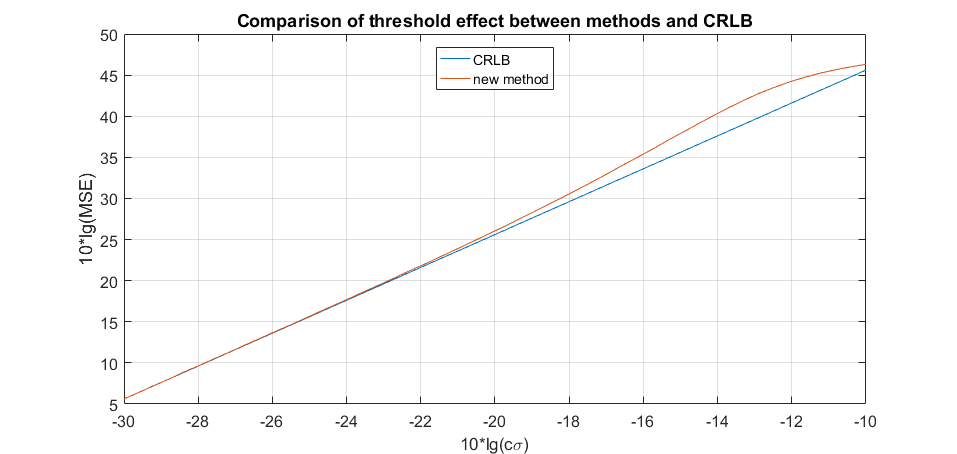
\includegraphics[scale=0.35]{fig4.JPG}
  \end{center}
  \begin{center} \textsc{Conclusions} \end{center}
  \begin{itemize}
    \item \small The proposed method performs only a little worse than the CRLB.
    \item \small The error thresholding effect doesn't occur until $ \sigma_d^2 = 0.0001 $
  \end{itemize}
\end{frame}
 
\end{document}
